\chapter{Metodología}\label{cap:metodologia}

\section{Formalización de ZSD} \label{ssec:formalizaciondezsd}
Para formalizar ZSD denotamos el conjunto de las clases como $\mathcal{C} = \mathcal{S} \cup \mathcal{U}$, donde $\mathcal{S}$ son las clases vistas para entrenamiento y $\mathcal{U}$ las clases no vistas, utilizadas en la etapa de pruebas. Además se tiene que $\mathcal{S} \cap \mathcal{U} = \emptyset$. Aunque no es necesario definir el conjunto de clases de pruebas, ya que el modelo tiene que ser capás de detectar tanto clases vista como las no vista, esto se hace para poder tener una evaluación cuantitativa.

Denotamos a una imagen como $\mathcal{I} \in \mathbb{D}^{\mathcal{M} \times \mathcal{N} \times 3}$. Donde $\mathbb{D} = \{0,...,255\}$, $\mathcal{M}$  es el largo de la imagen, $\mathcal{N}$ el ancho. Esta es la forma en la que se representa cada pixel de la imagen en el formato \textbf{RGB}, donde se tiene 3 canales que caracterizan la intensidad de los colores rojo, verde y azul. 

Por cada imagen se provee un conjunto de cuadros delimitadores  $\mathbb{B} = \{b_0,...,b_k\mid b_i \in N^4\}$ y sus etiquetas asociadas como $\mathbb{Y} = \{y_0,...,y_k\mid y_i \in \mathcal{C}\}$. Para cada cuadro delimitador $b_i$ extraemos una característica profunda utilizando una red neuronal convolucional denotada como $\phi(b_i) \in \mathbb{R}^{D_1}$. 

Denotamos las incrustaciones semánticas $w_j \in  \mathbb{R}^{D_2}$ obtenido por algún modelo como Wor2Vec. El conjunto de todas las imágenes de entrenamiento se indica con $\mathcal{X}^s$, que contiene ejemplos de todas las clases de objetos visibles.  El conjunto de todas las imágenes de prueba que contienen muestras de clases de objetos invisibles se indica con  $\mathcal{X}^u$. En particular, no hay ningún objeto de clase invisible en $\mathcal{X}^s$, pero $\mathcal{X}^u$ puede contener objetos vistos.\\

El objetivo es encontrar una matriz de proyección $W_p$, tal que \[ \psi_i = W_p\phi(b_i) \:\:\:\mid\:\:\: W_P \in \mathbb{R}^{D_2 \times D_1},\:\:\: \psi_i \in \mathbb{R}^{D_2} \] Note que $\psi_i$ y las incrustaciones semánticas se encuentran en el mismo dominio. Como mencionamos en secciones anteriores, el espacio vectorial semántico, tiene una gran capacidad de capturar similitudes semánticas. Por lo cual, resulta clave encontrar una matriz que para cada cuadro delimitador se proyecte lo mas cerca posible a la incrustación semántica de su clase. 

El resultado es una función \[f : \mathcal{X}, W_p  \to \{y_0,...,y_k\mid y_i \in \mathcal{C}\} \quad \operatorname{con}\quad \mathcal{X} =  \mathcal{X}^s \cup \mathcal{X}^u\] con un riesgo empírico regularizado mínimo definido de la siguiente manera $\mathcal{R}$ de la siguiente manera: \[ \arg_{}\min_{f \in F} \mathcal{R}(f(x,W_p))\quad, \] donde $x \in \mathcal{X}^s$ durante el entrenamiento. La función de mapeo utilizada en la etapa de inferencia, tiene la siguiente forma \[ f(x,W_p) = \arg_{}\max_{y \in \mathcal{C}}\max_{b \in \mathbb{B}(x)} (F(x,y,b,W_p)) \quad,\] donde los $\mathbb{B}(x)$ es el conjunto de propuestas de la imagen $x$. Intuitivamente se buscan los cuadros delimitadores de mejor puntuación y se les asigna la categoría de objeto de puntuación máxima.

\section{Arquitectura y Diseño} \label{sec:arquitecturaydiseno}

\subsection{Arquitectura} \label{ssec:arquitectura}
\begin{figure}
	\centering
	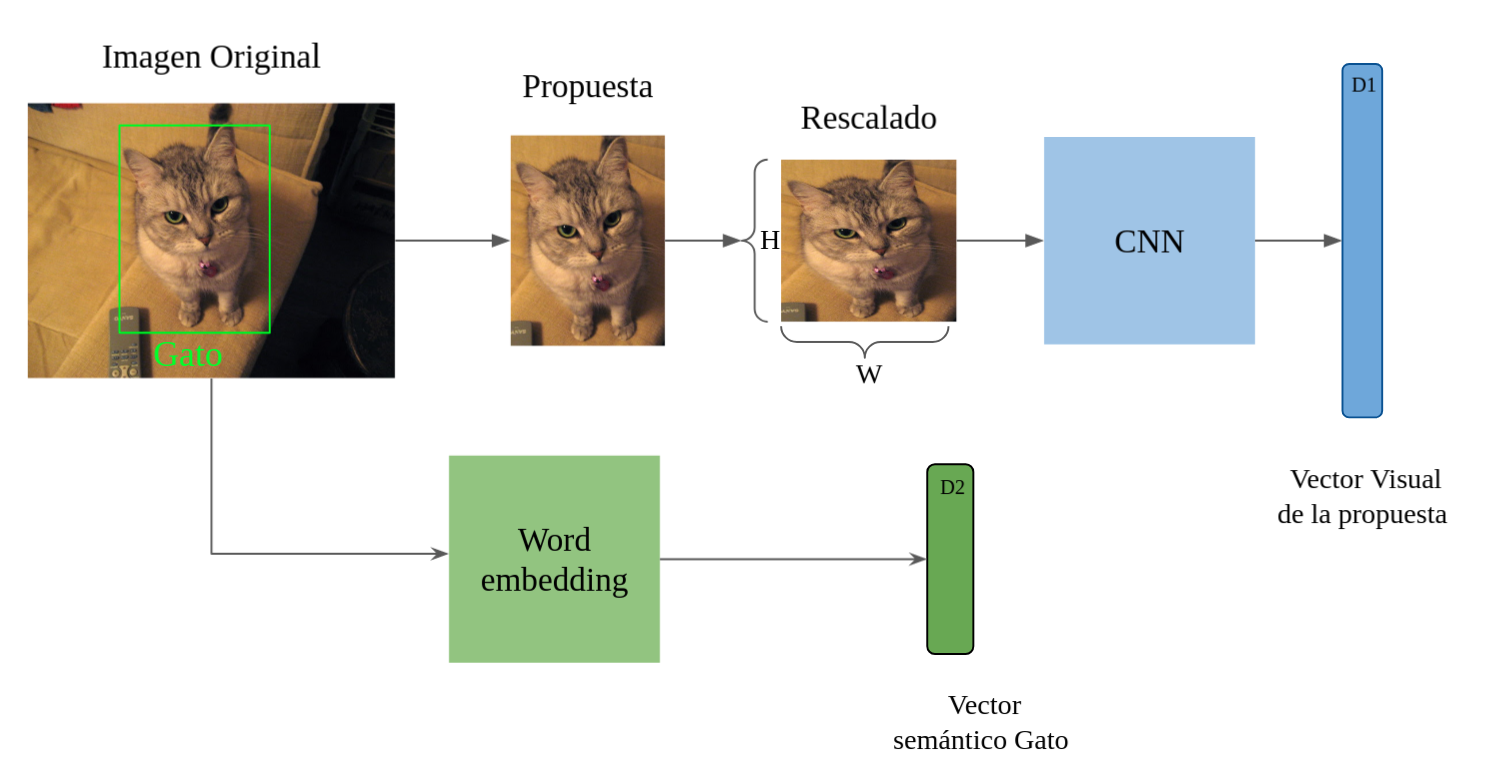
\includegraphics[width=0.9\textwidth]{img/arquitectura.png}
	\caption{Arquitectura propuesta y la dimensión de cada paso.}
	\label{fig:arqutectura}
\end{figure}
Como ya mencionamos anteriormente decidimos basarnos en el modelo propuesto por Ankan Bansal \cite{bansal2018zero}. Su arquitectura propuesta se puede dividir en las siguientes etapas.
\begin{itemize}
	\item \textbf{Pre-procesamiento:} Por cada imagen de entrenamiento, se extrae por cada cuadro delimitador una característica profunda utilizando una red neuronal convolucional y se asocia con el vector semantico a la clase que corresponde dicho cuadro, que se puede obtener de modelos de incrustación de palabras previamente entrenados como Glove o Word2vec. Esta etapa nos genera como salida dos listas $X = [\phi(b_0),...,\phi(b_k) \mid \phi(b_i) \in \mathbb{R}^{D_1}]$ $W = [w_0,...,w_k \mid w_i \in \mathbb{R}^{D_2}]$
	\item \textbf{Entrenamiento:} Utilizamos el espacio de incrustación común (${R}^{D_2}$) para calcular una medida de similitud entre las proyecciones  $\phi(b_i)$ y las words embedding $w_i$. Luego se entrena la proyección usando una pérdida de margen máximo que impone la restricción de que el puntaje de similitud de un cuadro delimitador con su clase verdadera debe ser más alto que el de otras clases. Para esto se utiliza una función de perdida definida como: \[\mathcal{L}(\psi_i, w_i) = \sum_{j \in \mathcal{S}, j\neq i} max(0, m - S_{ii} + S_{ij})\] $m$ es el margen máximo, y $S_{ij}$ es la similitud entre la proyección $i$-$esima$ y la incrustación $j$-$esima$. En la Figura \ref{fig:arqutectura}, se puede apreciar la arquitectura completa.
	 
	 También se agrega una función de pérdida de reconstrucción como sugiere Kodirov en \cite{kodirov2017semantic}. Se utilizan las características del cuadro delimitado proyectada para reconstruir las características profundas originales y calcular la pérdida de reconstrucción como la distancia $L2$  entre la característica reconstruida y la característica profunda original. \[\mathcal{L}_r = \Vert{\phi(b_i) - \psi_iW_p^T}\Vert^2 \] Luego definimos $\lambda$ como un coeficiente de ponderación que controla la importancia del primer y segundo término, que corresponden a las pérdidas de proyección y reconstrucción, respectivamente. Por lo cual la función de perdida total es: \[\mathcal{L}_t = \lambda \mathcal{L} + (1-\lambda) \mathcal{L}_r \]
	\item \textbf{Evaluación:} Por cada imagen del conjunto de entrenamiento, se genera un conjunto de propuestas de cuadros delimitadores. Luego, se eliminan todos lo que no tienen un puntaje de confianza mayor a un umbral. Para cada cuadro se computa la característica profunda $\phi(b_i)$ y utilizando la matriz $W_p$, para predecir las característica semántica. Por ultimo, se calcula la similitud con todas las características semántica, asignando al nuevo cuadro delimitador la que tenga mayor puntaje.
\end{itemize}
Es común que en la detección de objetos incluyan una clase de fondo para aprender un detector robusto que pueda discriminar eficazmente entre objetos de primer plano y objetos de fondo. En ZSD, esto no es un problema trivial, ya que no sabemos si un cuadro de fondo incluye elementos de fondo como cielo, tierra, bosque, etc. o una instancia de una clase de objeto invisible. En muchos trabajamos se proponen distintas técnicas para abordar este problema, pero no presentan mejoras en evaluaciones cuantitativas. Es por esto que no se incluye una arquitectura que discrimine cuadros de fondos.

Las propuestas de cuadro delimitadores son claves a la hora de evaluar un modelo, como mencionamos en secciones anteriores.  Muchas arquitecturas incluyen una red de propuestas regionales, RPN por sus siglas en ingles. De esta manera entrenan un modelo completo que también aprende a generar propuestas. Por lo que se pudo investigar, en nuestro caso resulta mas conveniente utilizar un modelo pre-entrenado como Edge-Boxes o Selective search.

\subsection{Conjuntos de datos} \label{ssec:conjuntosdedatos}
COCO es un conjunto de datos de detección, segmentación y subtítulos de objetos a gran escala. COCO tiene varias características: Segmentación de objetos,  Reconocimiento en contexto,  Segmentación de material de superpíxeles, 330 mil imágenes ($>$ 200 mil etiquetadas), 1,5 millones de instancias de objetos y 80 categorías de objetos.

 La gran cantidad de instancias de objetos y de categorías, resulta en un conjunto ideal para entrenar y evaluar modelos de ZSD. Ademas la mayoría de la imágenes consta de una gran cantidad de objetos que generan un contexto y no de uno solo centralizado, como son por ejemplo las imágenes del conjunto Visual Genome Dataset. Utilizamos las imágenes de entrenamiento del conjunto COCO 2014 e imágenes del conjunto de validación para realizar pruebas.
\\
Como COCO no provee una separación de los datos para evaluar modelos de ZSD, es necesario crear una forma de dividirlos. Notar que resulta de suma importancia dividir las clases, de tal manera que para todo objeto del conjunto prueba se encuentre otro similar en entrenamiento. Ademas, no se puede encontrar ningún objeto de prueba en los datos de entrenamiento. Dicho esto, se propuso una manera de separar las imágenes. COCO también tiene agrupada las clases por ``Clases superiores''
\begin{figure}[H]
	\begin{center}
	\centering
	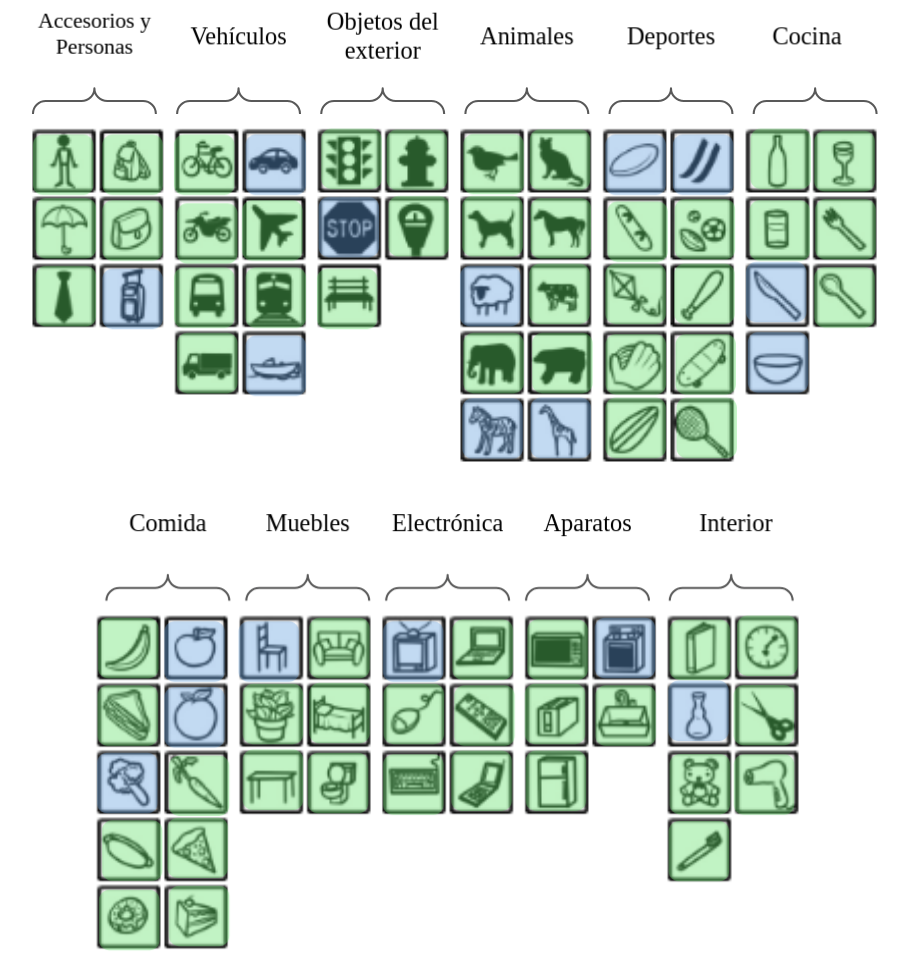
\includegraphics[width=0.9\textwidth]{img/data_set.png}
	\caption{Divisional de las clases para entrenamiento (verde) y pruebas (azul).}
	\label{fig:data_set}
	\end{center}	
\end{figure}
Por cada ``Clase superior'', elegimos de forma aleatoria un 70\% de clases para entrenamiento y un 30\% para pruebas. Es decir 47 y 18 clases respectivamente. En la Figura \ref{fig:data_set} se puede ver como quedan divididas. Por ultimo se eliminaron todas las imágenes de entrenamiento que contengan al menos una instancia de las clases de prueba. Esto resulta en 42564 imágenes con 261258 instancias de entrenamiento y 3008 con 10878 instancias de prueba. Bansal \cite{bansal2018zero}, divide el conjunto de datos, de manera similar, utiliza la misma cantidad de clases para pruebas y entrenamiento. Pero para crear las metaclases utiliza las incrustaciones de vectores de palabras para todas las clases y las agrupa en grupos de 10 usando la similitud de coseno entre los vectores de palabras como métrica. Por los problemas mencionados en la \autoref{sec:detecciondeobjetopordisparocero}, también utilizamos esta separación, de esta manera logramos una comparación de modelos mas justa.

\begin{figure}[H]
	\begin{center}
	\begin{subfigure}{.3\textwidth}
		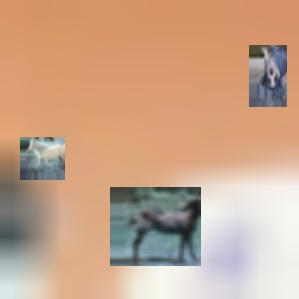
\includegraphics[width=0.85\textwidth]{img/cifar-zsd-test400.jpg}
		\label{fig:ex1}
	\end{subfigure}
	\begin{subfigure}{.3\textwidth}
		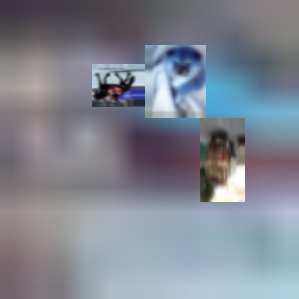
\includegraphics[width=0.85\textwidth]{img/cifar-zsd-test379.jpg}
		\label{fig:ex2}
	\end{subfigure}
	\begin{subfigure}{.3\textwidth}
		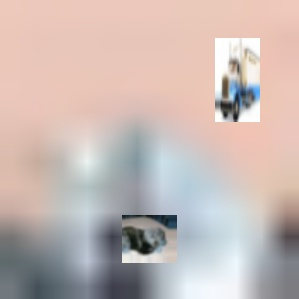
\includegraphics[width=0.85\textwidth]{img/cifar-zsd-test283.jpg}
		\label{fig:ex3}
	\end{subfigure}
	\caption{Ejemplos de imágenes del conjunto de datos CIFAR-ZSD.}
	\label{fig:CIFAR-ZSD}
	\end{center}
\end{figure}

COCO puede resultar pesado lo cual implica mucho tiempo de cómputos, para soluciona esto se creo un conjunto de datos sintéticos basado en CIFAR-100 datasets, el cual denominamos CIFAR-ZSD. Consta de imágenes localizadas, rotadas y re-escalada aleatoriamente con un fondo de otra imagen. Con esto se intenta simular imágenes reales en la cual un objeto puede aparecer con distintos aspectos y escalas. Este conjunto esta divido para que ninguna instancia de prueba  aparezca en el conjunto de entrenamiento.

Aunque resulta muy útil para probar modelos, no es bueno para reportar métricas reales. Pero en combinación con COCO, que si lo es, ambos cooperan para enfrentar el problema de ZSD de una forma mas practica.

\subsection{Detalles de la implementación} \label{ssec:detallesdelaimplementacion}

El paper de Bansal \cite{bansal2018zero}, carece de una implementación de acceso publico, por lo cual se realizo una implementación propria, basándose en los detalles que se pueden extraer del documento publicado. Fue necesario algunas presunciones, pero también, nos otorgo flexibilidades a la hora de codificar. Se busco obtener los resultados mas cerca a los reportados, pero siendo lo mas fiel a la información disponible. Para esto se decidió utilizar Python 3 con el framework Keras ejecutadose sobre TensorFlow.\\

Primero se realiza un preprocesamiento a todas las imagines del conjunto de datos de entrenamiento, que consiste en generar propuestas de objetos utilizando \textbf{Edge Boxes} o \textbf{Selective Search}. En el \autoref{cap:experimentos} se muestra los resultados de usar cada algoritmo. Luego por cada propuesta se calcula la intersección sobre unión con todos los cuadros delimitadores verdaderos. Si el IoU $> 0.5$ con algún cuadro verdadero, se guarda la propuesta y se la asocia con la clase del cuadro delimitador verdadero. Este preprocesamiento aumenta significativamente la cantidad de instancias para la etapa de entrenamiento. Resulta en un total de 1.436.835 instancias para COCO y 137.204 para CIFAR-ZSD. El siguiente paso consiste en generar el vector de características visuales y semánticas de cada cuadro delimitador. Como las CNN, utilizan un tamaño de entrada fijo, es necesario rescalar todos los cuadros.  Para \textbf{VGG16} utilizamos $224 \times 224$  y $299 \times 299$ en \textbf{Inception ResNet V2}, que son las dimensiones por defecto. El tamaño del vector de salida de cada red es de 512 en VGG y 1536 ResNet. Para ambas usamos pesos preentrenado en \textbf{Imagenet}. Este paso es diferente a como se hace en el paper de Bansal \cite{bansal2018zero}, ya que en este trabajo el modelo se entrena de extremo a extremo, es decir los pesos de la CNN se ajustan en la etapa de entrenamiento. Para obtener las características semánticas, utilizamos \textbf{Word2Vec} previamente entrenado de Google. Que Incluye vectores para un vocabulario de 3 millones de palabras y frases que se entreno en aproximadamente 100 mil millones de palabras de un conjunto de datos de Google News. La longitud del vector resultante es de 300. Luego se guardan dos archivos por cada imagen, en uno se encuentran los vectores visuales de cada clase y en el otro los semánticos.\\

Por ultimo, para el entrenamiento, se creo una red con una sola capa oculta, una capa de entrada del tamaño del vector de características visuales y una de salida de la dimensión de las características semánticas. Lo cual resulta en 153.900 parámetros entrenables con \textbf{VGG16} y 461.100 con \textbf{Inception ResNet V2}. Como optimizador se utilizo Adam, sin ninguna activación, un taza de aprendizaje de 10e-3 y un tamaño del lote de 64 muestras. Para la función de perdida se uso un lambda de 10e-3 y un margen máximo de 1.\\


\section{Experimentos}\label{cap:experimentos}

\subsection{Experimentación con propuesta de objetos} \label{ssec:experimentacionconpropuestadeobjetos}
\begin{table}[]
	\centering
	\resizebox{12.5cm}{!} {
		\begin{tabular}{|l|c|r|r|r|c|r|}
			\hline
			\textbf{}                     & \multicolumn{4}{c|}{\textbf{Edge Boxes}}                                                                                                   & \multicolumn{2}{c|}{\textbf{Selective Search}}               \\ \hline
			\textbf{Algoritmo}            & \multicolumn{4}{c|}{\textbf{-}}                                                                                                            & \textbf{Single}         & \multicolumn{1}{c|}{\textbf{Fast}} \\ \hline
			\textbf{Numero de propuestas} & \textbf{100}                 & \multicolumn{1}{c|}{\textbf{500}} & \multicolumn{1}{c|}{\textbf{1000}} & \multicolumn{1}{c|}{\textbf{5000}} & \textbf{$\approx$ 5000} & \multicolumn{1}{c|}{\textbf{$\approx$ 1000}}  \\ \hline
			Tiempo promedio (s)           & \multicolumn{1}{r|}{0.11}    & 0,11                              & 0.12                               & 0,12                               & \multicolumn{1}{r|}{5,48}   &         1,41                           \\ \hline
			Propuetas Totales             & \multicolumn{1}{r|}{4.415.244} & 22.050.071                          & 43.802.935                           & 161.809.194                          & \multicolumn{1}{r|}{350.535.591}   &   95.643.172                                 \\ \hline
			Propuestas con IOU $> 0.5$    & \multicolumn{1}{r|}{86.233}   & 133.942                            & 155.584                             & 194.891                             & \multicolumn{1}{r|}{221.551}   & 203.563                                   \\ \hline
		\end{tabular}
	}
	\caption{Resultados de correr los distintos algoritmos de propuestas de regiones en los datos de entrenamiento. El numero de propuestas verdaderas es 261.258.}
	\label{tab:edgeVSselct}
\end{table}

Como se menciono anteriormente, el numero de propuestas es un parámetro clave. Algunas métricas son muy sensible a la cantidad de propuestas, afectando los resultados finales. Esto surgió, cuando se obtuvieron las primeras métricas, los valores estaban muy lejos de los esperados, y a medida que se aumentaba la cantidad de propuesta, los resultados empeoraban. Por este motivo se probaron dos algoritmos (\textbf{Edge Boxes} y \textbf{Selective Search}) con algunas combinaciones de sus parámetros. Con el objetivo de obtener una cantidad de propuestas que se superponga con el mayor numero de objetos sin afectar las métricas.\\

Para no sesgar al experimento con los datos de de prueba, se definió la metodología de la siguiente manera. Por cada imagen de entrenamiento se corrió el generador de propuestas, se calculo el tiempo y la cantidad de cuadros verdaderos que tenían un IoU $> 0.5$, con algún cuadro verdadero. El tiempo es un parámetro importante ya que algunos algoritmos soy muy lentos y resulta imposible usarlos. Como se puede observar en el Cuadro \ref{tab:edgeVSselct}, \textbf{Selective Search} obtiene una mayor cantidad de superposición, pero con un numero exageradamente grande de propuestas. La mejor opción es usar \textbf{Edge-boxes}. En cuanto numero de propuestas totales resulta mas conveniente entre 100 y 500 propuestas como máximo, ya que al aumentar este numero no se generan mejoras en superposición pero si aumenta el numero de propuestas. Si tenemos en cunta el tiempo, resulta mejor \textbf{Edge-boxes}, ya que demora una fracción de lo que tarda \textbf{Selective Search}.\\

\subsection{Experimentación con CNN} \label{ssec:experimentacionconcnn}
Se deicidio analizar la CNN ya que el modelo final e muy dependiente de esta red y su capacidad de extraer caracteristicas visuales. Lo que se quiere aquí es que la red sea capas de asociar las caracteristicas visuales de objetos similares, y diferenciar los elementos de distinta naturaleza. En otras palabras, el espacio resultante tiene que distribuirse de tal manera que por ejemplo las imágenes de los animales estén muy cerca y a su ves alejado de vehículos o electrodomésticos, pero también tiene que mantener una separación entre los distintos animales como perro y gato. Bansal en su trabajo, propone utilizar \textbf{Inception ResNet V2}, pero esta red puede resulta muy pesada en cuanto a tiempo de ejecución y memoria. Por este motivo se decidió intentar con \textbf{VGG16}, que reduce el número de parámetros en las capas convolucionales y mejorar el tiempo de ejecución, ademas es una de la mas utilizada.\\

El experimento consistió en comparo miles de recuadros de 3 clases de entrenamiento, caballo, perro y camión.  Por cada cuadro se genero el vector de caracteristicas visuales. Luego se comparo utilizando la similitud coseno, entre todas las caracteristicas de caballo vs caballo, caballo vs camión y caballo vs perro. Se graficaron (Figura \ref{fig:vgg-vs-resnet}) las frecuencias de los resultados para cada CNN. Con esto se intenta observar como se distribuyen en el espacio visual, las distintas clases. Como se esperaba la similitud entre entre animales es mas grande que con un vehiculo. Pero, se observo que para \textbf{Inception ResNet V2} existe una mayor separación entre clases, aunque sus similitudes están mas dispersas. \textbf{VGG16}, parece tener una menor dispersión, pero la similitud coseno entre distintas clases tiene valores muy cercanos. Esto puede afectar de manera negativa ya que camión y caballo no poseen una gran diferencia y el modelo podría interpretarlo como clases similares.\\

% para generar tablas de latex
\begin{figure}
	\centering
	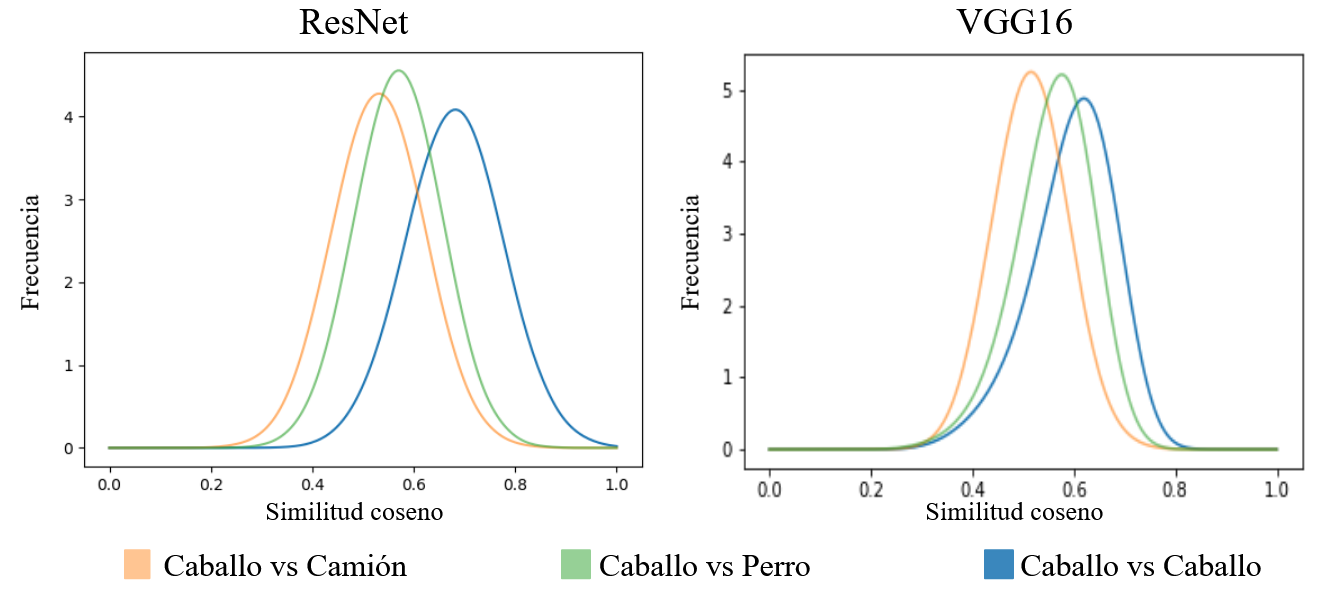
\includegraphics[width=1\linewidth]{img/vgg-vs-resnet}
	\caption{Frecuencia de la similitud coseno de los vectores de caracteristicas visuales, ente la misma y distintas clases, para las CNN  \textbf{Inception ResNet V2} y \textbf{VGG16}.}
	\label{fig:vgg-vs-resnet}
\end{figure}

\subsection{Definición de métricas} \label{ssec:definiciondemetricas}
Entre los diferentes conjuntos de datos anotados utilizados por los desafíos de detección de objetos y la comunidad científica, la métrica más común utilizada para medir la precisión de las detecciones es el  \textbf{Mean Average Precision (mAP)}, seguida por \textbf{Recall}. Un problema que tienen la métricas en detección de objetos, es la fata de una implementación estándar para calcularlas. Ademas, aquellas implementaciones publicas, están muy encapsuladas al código y resulta muy difícil adaptarlo, para medir rendimientos de modelos propios. Como ya se menciono, el código de Bansal \cite{bansal2018zero} no esta disponible, por este motivo fue necesario encontrar alguna implementación de estas métricas. Se encontraron varias y luego de hacer cambios para utilizarlos, los resultados variaban mucho de un código a otro.
Fue asi que se encontró el trabajo de Padilla Rafael \cite{padilla2020survey}, que explica lo planteado:\\

\begin{center}
	\textit{``La falta de consenso en diferentes trabajos e implementaciones de AP es un problema al que se enfrentan las comunidades académicas y científicas. Las implementaciones métricas escritas en diferentes lenguajes y plataformas computacionales generalmente se distribuyen con los conjuntos de datos correspondientes que comparten una descripción determinada del cuadro delimitador. De hecho, estos proyectos ayudan a la comunidad con las herramientas de evaluación, pero exigen trabajo adicional para adaptarse a otros conjuntos de datos y formatos de cuadro delimitador.''}\\
\end{center}

Ademas Padilla, propone una definición y un código para estandarizar las métricas, de esta manera se pueden comprar distintos modelos, de una forma ``justa''. Por estos motivos decidimos utilizar este trabajo, aunque los resultados de nuestros modelos, no sean exactos a los reportados por Bansal \cite{bansal2018zero}.\\

Ahora definamos las métricas, basándonos en el trabajo \cite{padilla2020survey}. Primero es necesario, estandarizar cuando un cuadro es:
\begin{itemize}
	\item Falso negativo (\textbf{FN}): No se obtuvo ninguna detección en absoluto, o para un cuadro delimitador verdadero el IoU $> umbral$ , y no se predijo correctamente la clase.
	\item Falso positivo (\textbf{FP}): Para un cuadro delimitador verdadero, se predijo correctamente la clase pero el IoU $< umbral$, o es un predicción duplicada, es decir, ya se marco otra con mayor IOU como \textbf{TP}.
	\item Verdadero positivo (\textbf{TP}): Para un cuadro verdad, se obtuvo un IoU $> umbral$ con algún cuadro verdadero y se predijo correctamente la clase.
	\item Verdadero negativo (\textbf{TN}): Esto solo tiene sentido si, se quisiera medir propuestas que no tenían un IoU $> umbral$ con todos los cuadros verdaderos, y ademas se predijo como clase de fondo. Pero en este trabajo no es utilizada.
\end{itemize}
El umbral por lo general es 0.5, pero se puede cambiar para exigir que tenga una mayor superposición.\\


La \textbf{Recall}, también conocida como sensibilidad, mide la probabilidad de que los objetos verdaderos (los que se encuentran en la imagen) se detecten correctamente, viene dado por: \[Recall =\frac{TP}{FN+TP}\] El trabajo de Bansal, define Recall de la siguiente manera: 
\begin{center}
	\textit{``Un cuadro delimitador predicho se marca como verdadero positivo solo si tiene una superposición de IoU mayor que un cierto umbral t con un cuadro delimitador de verdad del terreno y no se ha asignado ningún otro cuadro delimitador de mayor confianza al mismo cuadro de verdad del terreno. De lo contrario, se marca como falso positivo.''}\\
\end{center}

Sin poner en tela de juicio, si esto esta bien o mal, es claro que de esta forma solo se tiene en cuenta, los objetos que tuvieron al menos una propuesta con un IoU $> 0.5$ y el resto, quedan fuera del calculo de esta métrica. Esto genera una diferencia enorme en los resultados y dificulta la tarea de comprar con otros modelos, es  por esto que en este trabajo reportamos ambas. Bansal ademas, calcula una variación denominada K@Recall, donde solo se tienen en cuentan las K mejores propuestas basándose en la confianza de la predicción y el resto son descartadas.\\

\begin{equation} 
\label{eqn:precision}
Precision =\frac{TP}{FP+TP}
\end{equation}

AP, es una métrica popular para evaluar la precisión de los detectores de objetos mediante la estimación del área bajo la curva (AUC) de la relación \textbf{precisión} \ref{eqn:precision} x \textbf{recall}. La curva de \textbf{precisión} x \textbf{recall} puede verse como una compensación entre ambas métricas para diferentes valores de confianza asociados a los cuadros delimitadores generados por un detector. Si la confianza de un detector es tal que su FP es bajo, la precisión será alta. Sin embargo, en este caso, se pueden pasar por alto muchos aspectos positivos, lo que produce un FN alto y, por lo tanto, una recall baja. Por el contrario, si uno acepta más positivos, el recuerdo aumentará, pero el FP también puede aumentar, disminuyendo la precisión. Sin embargo, un buen detector de objetos debe encontrar todos los objetos reales  mientras identifica solo los objetos relevantes . Por lo tanto, un detector de objetos en particular puede considerarse bueno si su precisión permanece alta a medida que aumenta su recuperación, lo que significa que si el umbral de confianza varía, la precisión y la recall seguirán siendo altas. Por lo tanto, un área alta bajo la curva (AUC) tiende a indicar tanto una alta precisión como una alta recuperación. \textbf{mAP} para la detección de objetos es el promedio del AP calculado para todas las clases. Por lo general también se indica sobre que IoU se calcula, por ejemplo, mAP@0.5, o un conjunto de umbrales como mAP@[x, y]. El trabajo de Bansal reporta \textbf{mAP}, pero no indica sobre que IoU se calcula, a si que se asume que utilizo un valor de 0,5. Muchos trabajos que utilizan COCO, reportan mAP@[.5, .95]. Esta métrica resulta muy útil si se quiere comparar rendimientos entre distinto trabajos.


\subsection{Detalles de metodología de evaluación} \label{ssec:detallesdemetodologiadeevaluacion}
El principal experimento consto en replicar los resultados de Bansal \cite{bansal2018zero}. No se realizo exactamente sus experimentos, ya que esto no aportaría nada nuevo. Así que, se decidió analizar sus resultados y solo replicar los que consideramos indispensable y que seria un buen punto de partida. Por ejemplo, los experimentos con clases de fondo, no obtuvieron buenos resultados, en comparación con los que no la utiliza. Es por esto que no consideramos realizaros. El principal objetivo fue obtener un modelo que obtenga resultados lo mas similar posible a los reportados. Después de varias iteraciones, no se pudo lograr, y el principal motivo es la falta de una implementación para calcular las métricas. Se utiliza el código desarrollado por \cite{padilla2020survey}, pero sin ninguna garantía de que las métricas se calculen de la misma manera.\\

Ahora definamos la metodología de evaluación. El primer paso consiste generar propuestas para cada imagen, luego cada cuadro propuesto es reescalado al tamaño de la capa de entrada que tiene la CNN, y se le extrae el vector de características visuales. Después, se utiliza el modelo entrenado para inferir el vector de características semánticas, y se calcula la similitud coseno con los vectores semánticos de todas las clases o solo las invisibles, dependiendo si se quiere evaluar ZSDG o ZSD. Aquella clase que obtenga el mayor puntaje es asignada a la propuesta. También, se guarda la puntuación como la confianza de predicción.  Por ultimo, se agrupan todas las propuestas que se tengan asignada la misma clase y se corre un algoritmo de supresión no máxima. NMS elimina las predicciones repetidas y retorna las mejores propuestas de cada grupo. Al final obtenemos como resultado un conjunto de propuestas, sus clases y su respectivo puntaje. Estos datos se guardan en un archivo y luego se corre la implementación de Padilla, para obtener los resultados de las métricas.\\
